\documentclass[oneside, astronomy, noacknowlegments]{BYUPhys}

% Your name
  \Author{[Student Name]}

% Enter the date your thesis is approved
  \Year{[Year]}
  \Month{[Approval Month]}

% If you have a long title, split it between multiple lines using the \\ command
  \Title{[Title: Titles Must Be in Mixed Case and May Not Exceed Six Inches on One Line\\
  and Must Be in the Inverted Pyramid Format When\\
  Additional Lines Are Needed]
  }

% Your research advisor
\AdvisorTitle{Advisors}
  \Advisor{Justin Peatross and Michael Ware}

% For honors theses, enter the name of the honors Representative
  \HonorsRepresentative{Kristine Hansen}

% The text of your abstract
  \Abstract{ [The abstract is a summary of the thesis/dissertation
  with emphasis on the findings of the study. The abstract must not
  exceed 350 words in length and fit on one page, single spaced.] }

 \Keywords{[A comma-separated list of descriptive words for search purposes]}

% Acknowledge those who helped and supported you
  \Acknowledgments{
    [Acknowledgements should be simple, in good taste, and fit on one page]
  }

%% The members of your committee (masters only need A and B, PhD need all 4)
%  \MemberA{Committee Member A}
%  \MemberB{Committee Member B}
%  \MemberC{Committee Member C}
%  \MemberD{Committee Member D}
%

\begin{document}

 % Start page counting in roman numerals
 \frontmatter

 % This command makes the formal preliminary pages.
 % You can comment it out during the drafting process if you want to save paper.
 \makepreliminarypages

 % Make the table of contents.
 \tableofcontents

 % Start regular page counting at page 1
 \mainmatter

% OK. Everything is set up. Type your thesis here.

\chapter{A Sample Chapter}

\section{A Fascinating Section}
\label{sec:meaningfulname}

For a short thesis, you can usually just type the whole body of the
thesis here.  For longer documents you might consider typing
chapters in separate files and using the \verb|\include| command.
There is another example on the physics web page
(\href{http://www.physics.byu.edu/undergraduate/latex.aspx}{click
here to go there}) that shows how to do this.

You can create your bibliography right in the main tex document.
Here are references to a book \cite{Jackson1998}, an article
\cite{Peatross2000}, and a web site \cite{intel}. You can also use
BibTeX to keep track of your references.  The method for using
BibTeX is shown in the other example on the physics web page.

Making an index is easy. Just use the \verb|\index{Key}| command.
\index{Index!Making} You can include figures too (see
Fig.~\ref{fig:MirrorDiagram}).  Usually you need both eps and pdf
versions of each figure.
\begin{figure}
    \centerline{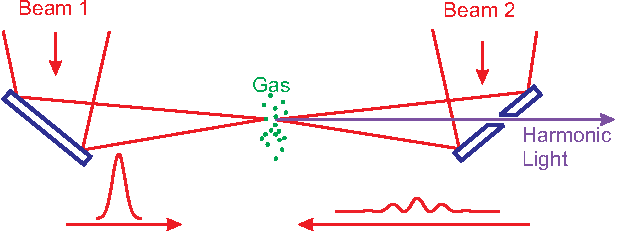
\includegraphics{Graphic1}}
    \caption[Setup for using counter-propagating light]{\label{fig:MirrorDiagram}
    A mirror with a hole is used to extract high-order harmonics generated in
    counter-propagating laser beams.}
\end{figure}

% Start labeling chapters with letters and calling them appendices
\begin{appendices}

\chapter{Appendix Title}
\label{sec:appendixname}

You can put supplimentary content in an appendix.

\end{appendices}

% Make the bibliography.
% Enter your references in the BibTex file "references.bib"
 \bibliography{references}

% Make the index
 \printindex

\end{document}
